\documentclass[]{article}
%\usepackage[a4paper, total={6.5in, 8.5in}]{geometry}
\usepackage{color}
\usepackage{hyperref}
\usepackage{amsmath}
\usepackage{amssymb}
\usepackage{graphicx}
\usepackage{float}
\usepackage{algorithm}
\usepackage{algpseudocode}
\usepackage{neurips_data_2023}

\title{Towards Comparable Active Learning}
\author{%
	Thorben Werner 
	\thanks{Information Systems and Machine Learning Lab (ISMLL)} 
	\\
	Institute of Computer Science\\
	University of Hildesheim\\
	Universitätsplatz 1, 31141 Hildesheim \\
	\texttt{werner@ismll.de} \\
	% examples of more authors
	\And
	Johannes Burchert$^*$ \\
	Institute of Computer Science\\
	University of Hildesheim\\
	Universitätsplatz 1, 31141 Hildesheim \\
	\texttt{burchert@ismll.de} \\
	\AND
	Prof. Lars Schmidt-Thieme$^*$ \\
	Institute of Computer Science\\
	University of Hildesheim\\
	Universitätsplatz 1, 31141 Hildesheim \\
	\texttt{schmidt-thieme@ismll.uni-hildesheim.de} \\
	% \And
	% Coauthor \\
	% Affiliation \\
	% Address \\
	% \texttt{email} \\
	% \And
	% Coauthor \\
	% Affiliation \\
	% Address \\
	% \texttt{email} \\
}

\begin{document}

\maketitle

\begin{abstract}
	Active Learning (AL) is a technique used in machine learning to improve data efficiency by selecting the most informative samples for annotation. 
	In this paper we address the issue of inconsistent results in active learning literature.
	Authors of previous papers are constantly reporting significant performance improvements in their original work, while subsequent literature fails to reproduce those results. This inconsistency leads to a chaotic landscape of AL algorithms.
	We propose the first AL benchmark that tests algorithms in all three major domains of tabular, image and text data.
	Furthermore, we discuss a central problem for reproducing AL experiments with the default seeding setup that depends on a single seed per experiment.
	...
\end{abstract}

\section{Introduction}
{\color{red} Version: 1.0}\\
Active Learning (AL) plays an important role in our society that applies machine learning to more and more areas and therefore has a high demand for labeled data in more and more areas.
A problem that concerns academic researchers and practitioners in businesses alike and even could be extended to education in schools and hobbyists around the world.
On top of providing a principled way to labeled unlabeled datasets, active learning is one of the two major approaches besides semi-supervised learning to make deep learning models more data efficient by requiring only a limited set of manually labeled data.
Both approaches are at their core orthogonal and can freely be combined and therefore we should continue our research efforts for both approaches. \\
Among others, the authors of \cite{zhou2021towards} have pointed out severe inconsistencies in results of AL papers in recent years. 
In their supplementary materials they conducted a meta analysis of reported results of several different AL algorithms and found that all considered algorithms only provided significant lifts in their own original papers, while all following literature reported performances no better that uncertainty sampling, or in some cases no better than random sampling for the same algorithm.
The result of these inconsistencies is a chaotic landscape of AL algorithms where every paper claims to archive state-of-the-art results by significantly outperforming everyone else, while the vast majority of results proves to be non-reproducible. \\ [1mm]
%
To allow comparison between 

\subsection{Contributions}
\begin{enumerate}
	\item Evaluation of Active Learning algorithms on datasets from 4 different domains, including synthetic data that highlights principled shortcomings of existing approaches.
	\item Novel experimental protocol for seeding the experiment with 3 different seeds to allow full control and reproducibility and analysis of how many restarts are required to converge to the true median performance reliably.
	\item Simple algorithm for an Oracle-Curve that can be constructed greedily and does not rely on search.
\end{enumerate}



%%%%%%%%%%%%%%%%%%%%%%%%%%%%%%%%%%%%%%%%%%%%%%%%%%%%%%%%%%%%%%%%%%%%%%%%%%%%%%%%%%
\section{Overview}
We constrain our work on pool-based active learning where a pool of unlabeled samples is fixed at the start of each experiment and samples are chosen sequentially.
Specifically, we are not experimenting on so-called batch active learning, where at each iteration multiple unlabeled samples are chosen at the same time.
Even though batch AL is the more active research domain, it does not have a principled advantage over single-sample AL except speed of computation.
Not only is the problem of optimizing a portfolio of unlabeled samples more complicated to solve, the algorithms also have systematically less information per sample to work with.
For this reason we propose to focus more research effort on single-sample AL to find better algorithms in an environment that is simpler to solve and easier to control.
Table \ref{tab:benchmark_comparison} shows a feature comparison between our proposed benchmark and several existing benchmarks in the literature, as well as methodological AL papers with experiments on at least two data domains.
\begin{table}[h]
	\centering
	\begin{tabular}{l | c c c c c}
		Paper & Sampling & \# Datasets & Domains & Algorithms & Oracle \\
		\hline
		Beck et al. \cite{beck2021effective} & batch & 4 & 1 & 7 & - \\
		Hu et al. \cite{hu2021towards} & batch & 5 & 2 & 13 & - \\
		Li et al. \cite{li2022empirical} & batch & 5 & 1 & 13 & - \\
		Zhou et al. \cite{zhou2021towards} & batch & 3 & 2 & 2 & \checkmark \\
		\textbf{Ours} & single & 9 & 4 & 6 & \checkmark 
	\end{tabular}
	\caption{Comparison of our benchmark with the existing literature}
	\label{tab:benchmark_comparison}
\end{table}

%Manual NIPS Benchmark paper eval (out of 6):
%\begin{itemize}
%	\item Has new method: 1
%	\item Multiple domains: 2
%	\item $> 5$ datasets: 3
%	\item $> 5$ baselines: 4
%\end{itemize}


%%%%%%%%%%%%%%%%%%%%%%%%%%%%%%%%%%%%%%%%%%%%%%%%%%%%%%%%%%%%%%%%%%%%%%%%%%%%%%%%%%
\subsection{Problem Description}
{\color{red} Version: 1.0}\\
Given two spaces $\mathcal{X}:=\mathcal{R}^M$ and $\mathcal{Y}:=\mathcal{R}^C$, a sample $\mathcal{D}_1,\ldots,\mathcal{D}_N \subseteq (\mathcal{X}\times \mathcal{Y})^*$ of sequences of pairs $(x,y)$  from an unknown distribution $p$ called datasets and a number $B\in\mathcal{N}$ with $B < |\mathcal{D}|$. \\
Given two functions $\ell:\mathcal{Y}\times \mathcal{Y}\rightarrow \mathcal{R}$ called loss, and $A: (\mathcal{X} \times \mathcal{Y})^* \times \mathcal{X}^* \rightarrow \mathcal{Y}^{\mathcal{X}}$ called learning algorithm, find a function
\begin{align*}
	a: (\mathcal{X}\times \mathcal{Y})^* \times \mathcal{X}^* \rightarrow \{0,1\}^*
	\quad\quad \text{\tiny (equivariant in the second argument)}
\end{align*}
% which is equivariant in the second argument, 
called acquisition function, s.t. the expected loss of a model learned on all predictors plus $B$ acquired targets is minimal:
\begin{align*}
	\mathbb{E}_{\mathcal{D}\text{train},\mathcal{D}\text{test}\sim p}   &
	% \frac{1}{|\mathcal{D}\text{test}|} \sum_{(x,y)\in\mathcal{D}\text{test}}
	% \operatorname{avg} \{
	%  \ell(y, \hat y(x)) \mid (x,y)\in\mathcal{D}\text{test} \}
	\operatorname{avg}\limits_{(x,y)\in\mathcal{D}\text{test}}
	\ell(y, \hat y(x)) 
	\\
	\text{with }
	\hat y:= & A( (\mathcal{D}\text{train}_{n_1},\ldots,\mathcal{D}\text{train}_{n_B}), \mathcal{D}\text{train}|_{\mathcal{X}})
	\\ 
	n_b := & \text{index}( a( (\mathcal{D}\text{train}_{n_1},\ldots,\mathcal{D}\text{train}_{n_{b-1}}), \mathcal{D}\text{train}|_{\mathcal{X}}) ),
	\quad b\in 1{:}B
\end{align*}
(\textit{We would need to switch from lowest expected loss to highest AUC}) \\
Since combinatorial problem of finding the optimal subset $\mathcal{D}_\text{train}$ is computational not feasible, we allow sequential construction of $\mathcal{D}_\text{train}$. \\
%
To construct the active learning setting from existing labeled datasets, we first split it into $\mathcal{D}_\text{train}$, $\mathcal{D}_\text{val}$ and $\mathcal{D}_\text{test}$ and then suppress the labels $\mathcal{Y}$ of $\mathcal{D}_\text{train}$ to form the unlabeled pool $\mathcal{U} := \mathcal{X}^*$ and form and initial labeled pool by uniformly sampling $k$ number of instances per class from $\mathcal{U}$ and recovering their label $\mathcal{L} := (\mathcal{X}, \mathcal{Y})^{k*C}$. \\
%
Following \cite{zhou2021towards}, the quality of an active learning algorithm is evaluated by an "anytime" protocol that incorporates classification performance at every iteration, not just the final performance after the budget is exhausted.
We employ the normalized area under the accuracy curve (AUC):
\begin{equation}\label{eq:auc}
	\operatorname{auc}(\mathcal{U}, \mathcal{L}, \hat y, B) := \frac{1}{B} \sum_{i=1}^{B} \operatorname{Acc}(y_{test}, \hat y_i(x_{test}))
\end{equation}
Where $\hat y_i$ is the retrained classification model after the i-\textit{th} instance was selected.

\begin{minipage}{0.49\linewidth}
	\begin{algorithm}[H]
		\caption{Oracle}\label{alg:oracle}
		\begin{algorithmic}[1]
			\Require $\mathcal{U}$ \Comment{Unlabeled Pool}
			\Require $\tau$ \Comment{Unlabeled Sample Size}
			\State $\mathcal{L}^{(1)} \gets \operatorname{seed}(\mathcal{U})$  %\Comment{Create the initial labeled set}
			\State $\mathcal{U}^{(1)} \gets \mathcal{U} \setminus \mathcal{L}^{(1)}$
			\For{$i := 1 \ldots B$} 
			\State $\text{acc}^{(i)} \gets \operatorname{Retrain}(\mathcal{L}^{(i)})$  %\Comment{$\operatorname{Retrain}(\mathcal{L}^{(i)})$ is shorthand for $\operatorname{Retrain}(\mathcal{L}^{(i)}, \mathcal{L}^\text{test}, \hat y_\theta, e^\text{max})$}
			\State $u^{(i)} \underset{\tau}{\sim} \text{unif}(1:|\mathcal{U}^{(i)}|)$
			\State $r* \gets 0$
			\For{$j := 1 \ldots \tau$} %\Comment{Testing every unlabeled point}
			\State $y^{(j)} \gets \operatorname{label}(u^{(i)}_{j})$
			\State $\mathcal{L}^{(j)} \gets \mathcal{L}^{(i)} \cup \{(u^{(i)}_j, y^{(j)})\}$
			\State $\text{acc}^{(j)} \gets \operatorname{Retrain}(\mathcal{L}^{(j)})$  
			\State $r^{(j)} \gets \text{acc}^{(j)} - \text{acc}^{(i)}$
			\If{$r^{(j)} > r^*$} %\Comment{Select point with largest increase in performance}
			\State $r* \gets r^{(j)}$
			\State $j* \gets j$
			\EndIf  
			\EndFor
			\If{$r^* = 0$}
			\State $j* \gets \operatorname{margin}(u^{(i)}, \hat y_\theta)$
			\EndIf
			\State $y^{(i)} \gets \operatorname{label}(u^{(i)}_{j*})$
			\State $\mathcal{L}^{(i+1)} \gets \mathcal{L}^{(i)} \cup \{(u^{(i)}_{j*}, y^{(i)})\}$
			\State $\mathcal{U}^{(i+1)} \gets \mathcal{U}^{(i)} \setminus \{u^{(i)}_{j*}\}$
			\EndFor
			\State
			\Return $\frac{1}{B} \sum_{i=1}^{B} \text{acc}^{(i)}$
		\end{algorithmic}
	\end{algorithm}
\end{minipage}
\hspace{3mm}
\begin{minipage}{0.5\linewidth}
	\begin{algorithm}[H]
		\caption{Retrain}\label{alg:retrain}
		\begin{algorithmic}[1]
			\Require $\mathcal{L}$ \Comment{Labeled Pool}
			\Require $\mathcal{D}_\text{val}$ \Comment{Validation Data}
			\Require $\mathcal{D}_\text{test}$ \Comment{Test Data}
			\Require $\hat y_\theta$ \Comment{Class. Model}
			\Require $e^\text{max}$ \Comment{Maximum Epochs}
			\State $\text{loss}^* \gets \infty$
			\For{$i := 1 \ldots e^{\text{max}}$}
			\State $\theta_{i+1} \gets \theta_i - \eta \nabla_\theta \ell(\mathcal{L}, \hat y_{\theta})$
			\State $\text{loss}_i \gets \ell(\mathcal{D}^\text{val}, \hat y_{\theta})$
			\If{$\text{loss}_i < \text{loss}^*$}
			\State $\text{loss}^* \gets \text{loss}_i$
			\Else
			\State Break
			\EndIf
			\EndFor
			\State
			\Return Acc($\mathcal{D}^\text{test}, \hat y_{\theta}$)
		\end{algorithmic}
	\end{algorithm}
	In Alg. \ref{alg:oracle} $\operatorname{Retrain}(\mathcal{L}^{(i)})$ is shorthand for $\operatorname{Retrain}(\mathcal{L}^{(i)}, \mathcal{D}_\text{test}, \hat y_\theta, e^\text{max})$, $\operatorname{label}(u^{(i)}_{j})$ recovers the label of instance $u^{(i)}_{j}$ and $\operatorname{margin}(u^{(i)}, \hat y_\theta)$ applies margin sampling to select as a fallback, when the oracle has not found another option that induces a positive change in classification performance.
\end{minipage}


%%%%%%%%%%%%%%%%%%%%%%%%%%%%%%%%%%%%%%%%%%%%%%%%%%%%%%%%%%%%%%%%%%%%%%%%%%%%%%%%%%
%%%%%%%%%%%%%%%%%%%%%%%%%%%%%%%%%%%%%%%%%%%%%%%%%%%%%%%%%%%%%%%%%%%%%%%%%%%%%%%%%%
%%%%%%%%%%%%%%%%%%%%%%%%%%%%%%%%%%%%%%%%%%%%%%%%%%%%%%%%%%%%%%%%%%%%%%%%%%%%%%%%%%
\section{Related Work}
{\color{red} Version: Braindump}\\
Many different algorithms have been proposed for active learning. 
In this work we focus on those approaches that have shown consistent results over the years as well as newer approaches that have demonstrated significant lifts in their initial experiments.
AL algorithms can be categorized into two classes: Geometric approaches and uncertainty-based approaches.
Geometric approaches include CoreSet \cite{sener2017active} and TypiClust \cite{hacohen2022active}, which use clustering techniques to partition the data and then sample their unlabeled points based on the clusters.
Uncertainty-based approaches include classic uncertainty sampling (based on Shannon-Entropy and the margin-score), BALD \cite{kirsch2019batchbald} and BADGE \cite{ashdeep}, which use metrics to measure the classifiers state. \\ [1mm]
%
Some previous work also aimed to provide a benchmark suite for active learning:
The authors of \cite{beck2021effective} and \cite{li2022empirical} both focus on active learning in the image domain.
While \cite{beck2021effective} discuss a new metric to measure AL performance, which they call "Label Efficiency" and provide experiments on many common configurations for data preparation, model training and other hyperparameters, \cite{li2022empirical} focuses on combined approaches of AL and semi-supervised learning to aid model training.
The authors of \cite{hu2021towards} study models that are learned with AL techniques in the image and text domain.
They test for several different properties of the models including robustness, response to compression techniques and final performance.


%%%%%%%%%%%%%%%%%%%%%%%%%%%%%%%%%%%%%%%%%%%%%%%%%%%%%%%%%%%%%%%%%%%%%%%%%%%%%%%%%%
%%%%%%%%%%%%%%%%%%%%%%%%%%%%%%%%%%%%%%%%%%%%%%%%%%%%%%%%%%%%%%%%%%%%%%%%%%%%%%%%%%
%%%%%%%%%%%%%%%%%%%%%%%%%%%%%%%%%%%%%%%%%%%%%%%%%%%%%%%%%%%%%%%%%%%%%%%%%%%%%%%%%%
\section{Methodology}

%%%%%%%%%%%%%%%%%%%%%%%%%%%%%%%%%%%%%%%%%%%%%%%%%%%%%%%%%%%%%%%%%%%%%%%%%%%%%%%%%%
\subsection{Evaluation}\label{sec:evaluation}
{\color{red} Version: 1.0}\\
We compare different AL algorithms based on their median AUC score (Eq. \ref{eq:auc}) across multiple restarts of the experiment.
Each restart will retain the train/test split (often given by the dataset itself), but introduces a new validation split to mimic the leave-one-out protocol for cross-validation.
The AUC incorporates performance in early stages (low budget) as well as capabilities to push the classifier in later stages (high budget).
A good AL algorithm should be able to perform well in both scenarios. \\ [1mm]
Since AUC is dependent on the chosen budget, we need a general rule on how to set this hyperparameter that does not inherently benefit a subset of algorithms.
In this work, we choose the budget per dataset to be the first point at which any algorithm (except oracle) manages to reach a percentage of the upper bound performance measured on the full dataset.
Even though we would like to propose a single percentage value for all datasets, we found that different data modalities and use cases need different percentages to produce sensible budgets.
We propose the following values: \textbf{Tabular}: 99\%, \textbf{Image}: 90\% and \textbf{Text}: 95\%. \\ [1mm]
Additionally, we provide evidence in Fig. \ref{fig:restarts} that previous works have not evaluated their experiments with a sufficient number of restarts.
To create Fig. \ref{fig:restarts} we used all our 50 runs from the margin/random sampling algorithm on the splice dataset.
From these 50 runs we uniformly sampled subsets of runs and calculated the median AUC for this subset.
One AUC value like this corresponds to one cross-validated experiment sampled from the distribution of experiments that are restarted exactly this many times.
To create one slice in Fig. \ref{fig:restarts}, we drew 50 samples from this distribution.
Each box-plot represents the variance of an evaluation if conducted with the respective number of restarts.
We can clearly observe that low repetitions ($<10$) provide an uncertain evaluation where lucky and unlucky draws of the same experiment give drastically different median AUC values.
\begin{figure}
	\centering
	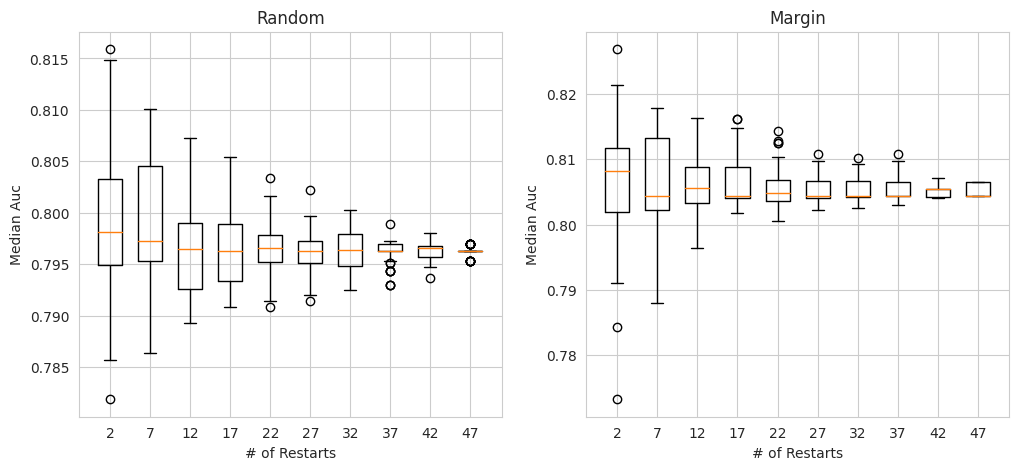
\includegraphics[width=\linewidth]{img/ablation_restarts.png}
	\caption{Random draws from an experimental distribution on the Splice datasets with different numbers of repetitions. Each point on the Y-axis represents a cross-validated result that could have been reported in a paper. This analysis shows the drastic differences in performance one could observe even when repeating an experiment 2-10 times.}
	\label{fig:restarts}
\end{figure}
To combat is uncertain evaluation, we propose to repeat every experiment 50 times, to arrive at the true median AUC for each algorithm.

%%%%%%%%%%%%%%%%%%%%%%%%%%%%%%%%%%%%%%%%%%%%%%%%%%%%%%%%%%%%%%%%%%%%%%%%%%%%%%%%%%
\subsection{Reproducibility}\label{sec:reproducibility}
{\color{red} Version: 1.0}\\
A big focus in this work is to provide an experimental setup that is fully reproducible independent of the dataset, classification model or AL algorithm used.
In our opinion, an evaluation on one dataset with a given seed should always be done on the same validation split as well as using the same random state for all included systems like the mini batch sampler for the classifier model training.
Even though different AL algorithms will pick different samples, making them unavailable for sampling in earlier or later batches, the theoretical decision tree for every possible choice in every iteration $i$ should stay the same.
Since every possible trajectory cannot be precomputed and stored to disk, we need to resort to seeding the evaluation.
The default choice of setting a global seed at the start of the experiment is not sufficient here, since a single additional random draw from the random number generator completely changes the behavior of all other systems.
This additional random number might be drawn during the initialization of the classification model, the AL algorithm, or even during every AL iteration if $\Omega$ is stochastic.
This problem also applies to the initialization of the classification model $\theta$ and the initialization and querying of $\Omega$.
The desired control over all these processes can only be archived by assigning a separate random number generator to all these processes.
To the best of our knowledge, we are the first work that discusses this issue and proposes a solution for it.
We hypothesize that the insufficient setup with global seeds contributes to the on-going problem of inconsistent results of AL algorithms in different papers. \\ [1mm]
In summary, we introduce three different seeds: $s_\Omega$ for the acquisition function, $s_\mathcal{D}$ for dataset splitting and mini batch sampling and $s_\theta$ for model initialization and sampling of dropout masks.
Unless stated otherwise, we will keep $s_\Omega$ fixed for restarts of the same experiment, while $s_\mathcal{D}$ and $s_\theta$ are incremented by 1 between restarts to introduce stochasticity into our framework.

%%%%%%%%%%%%%%%%%%%%%%%%%%%%%%%%%%%%%%%%%%%%%%%%%%%%%%%%%%%%%%%%%%%%%%%%%%%%%%%%%%
\subsection{Oracle}\label{sec:oracle}
{\color{red} Version: 1.0}\\
Posing active learning as a sequence ordering problem, the oracle sequence for a given combination of dataset, model and training procedure would be the sequence that induces the highest AUC score for a given budget.
However, since this combinatorial problem is not solvable for realistic datasets, previous works have proposed approximations to this oracle sequence.
\cite{zhou2021towards} has used simulated annealing to search for the optimal sequence and used the best  solution found after a fixed time budget. 
Even though their reported performance curves display a significant lift over all other algorithms, we found the computational cost of reproducing this oracle for all our datasets to be prohibitive (The authors reported the search to take several days per dataset on 8 V100 GPUs). \\
In this paper we propose a greedy oracle algorithm that constructs an approximation of the optimal sequence in an iterative fashion.
Our oracle simply tests every data point in the provided sample of unlabeled points by fitting the classifier and directly measuring the resulting validation performance.
The point with the best validation performance is selected and added to the labeled pool for that iteration.
We noticed that this oracle is overfitting on the validation set, resulting in stagnating or even decreasing performance curves in later AL iterations.
To circumvent this problem, we introduced margin sampling as a fallback option for the oracle.
Whenever the oracle does not find an unlabeled point that results in an increase in performance (indicating an overfitting position), it defaults to margin sampling in that iteration.
The pseudocode for our oracle can be found in Alg. \ref{alg:oracle}.


%%%%%%%%%%%%%%%%%%%%%%%%%%%%%%%%%%%%%%%%%%%%%%%%%%%%%%%%%%%%%%%%%%%%%%%%%%%%%%%%%%
%%%%%%%%%%%%%%%%%%%%%%%%%%%%%%%%%%%%%%%%%%%%%%%%%%%%%%%%%%%%%%%%%%%%%%%%%%%%%%%%%%
\section{Implementation Details}

%%%%%%%%%%%%%%%%%%%%%%%%%%%%%%%%%%%%%%%%%%%%%%%%%%%%%%%%%%%%%%%%%%%%%%%%%%%%%%%%%%
\subsection{Available Information}
At each iteration $i$ the AL algorithm needs to pick an unlabeled datapoint based on a fixed set of information $\{\mathcal{L}^{(i)}, \mathcal{U}^{(i)}, B, |\mathcal{L}^{(i)}|-|\mathcal{L}^{(1)}|, \text{acc}^{(i)}, \text{acc}^{(1)}, \theta^{(i)}, \text{opt}_\theta\}$, where $\theta^{(i)}$ is the current classifier and $\text{opt}_\theta$ is the optimizer used to fit $\theta^{(i)}$.
We allow algorithms to derive additional information of this set like predictions of the classifier, K-Means clustering or even training new classifiers.
However, the algorithm may not incorporate external information like other datasets, queries to recover additional labels, or the test/validation set.

%%%%%%%%%%%%%%%%%%%%%%%%%%%%%%%%%%%%%%%%%%%%%%%%%%%%%%%%%%%%%%%%%%%%%%%%%%%%%%%%%%
\subsection{Sampling Strategies}\label{sec:sampling_strategies}
We selected AL algorithms that have good performances reported by multiple different sources.
To ensure a fair comparison we fixed the training process of our classification model as well as the set of available information for the algorithm and selected only those that can work under these restrictions:
\paragraph{Uncertainty Sampling} 
Tries to find the sample that the classifier is most uncertain about. For our benchmark we use entropy and margin (a.k.a. best-vs-second-best) sampling.
\paragraph{BALD \cite{kirsch2019batchbald}}
Applies the query-by-committee strategy of model ensembles to a single model by interpreting the model's parameters as distributions and then sample multiple outputs from them via Monte-Carlo dropout.
\paragraph{BADGE \cite{ashdeep}} Uses gradient embeddings of unlabeled points to select samples where the classifier is expected to change a lot. The higher the magnitude of the gradient the higher is the expected improvement in model performance.
\paragraph{Coreset \cite{sener2017active}}
Employs K-Means clustering to try to cover all {\color{red}modalities (is this the right word?)} that are observed in the data.
Selects the unlabeled sample that is the furthest away from all cluster centers.
In this work we use the greedy variant of Coreset and we also encode the data with the current classifier $\theta_i$ before clustering.
\paragraph{TypiClust}
Relies on clustering similar to Coreset but proposes a new measure called "Typicality" to select unlabeled centers.
Tries to select points that are in the densest regions of clusters that do not contain labeled samples yet.
For this work we also use the current classifier $\theta_i$ to encode data if necessary (raw images or text).
%
\subsubsection{Honorable Mentions}
\paragraph{Learning Loss for AL}
Introduces an updated training of the classification model with an auxiliary loss and therefore cannot be compared fairly against classification models without this boosted training regime.

%%%%%%%%%%%%%%%%%%%%%%%%%%%%%%%%%%%%%%%%%%%%%%%%%%%%%%%%%%%%%%%%%%%%%%%%%%%%%%%%%%
\subsection{Choosing the Classifier}\label{sec:choosing_the_classifier}
Traditionally, the classifier is chosen per dataset so that it is capable of solving the dataset close to the SOTA performance reported in the literature.
Similar to our hypothesis in section \ref{sec:evaluation} we hypothesize that AL algorithms will perform similarly on small classifiers and more complex ones, so that the overall ranking of algorithms stays the same.
{\color{red} TODO: Transform this into full hypothesis incl. formatting?}\\
On the basis of this hypothesis we opt to use smaller classifiers that still solve the dataset to a reasonable degree.
Smaller classifiers also require fewer labeled datapoints to acquire performance close to the upper bound.
For every dataset the chosen architecture's hyperparameters are optimized by to archive maximum upper bound performance.
For an overview of architectures and hyperparameters please refer to Appendix \ref{app:hyperparameters}.


%%%%%%%%%%%%%%%%%%%%%%%%%%%%%%%%%%%%%%%%%%%%%%%%%%%%%%%%%%%%%%%%%%%%%%%%%%%%%%%%%%
\subsection{Training the Classifier}\label{sec:training_the_classifier}
{\color{red} Version: 0.1}\\
Generally, the classification model can be trained in two ways. Either you reset the parameters after each AL iteration and train the classifier from scratch with the updated labeled set $\mathcal{L}^{(i)}$, or you retain the previous state and only fine-tune the classifier on $\mathcal{L}^{(i)}$ for a reduced number of epochs.
In this work we use the fine-tuning method for raw datasets to save computation, while we use the from-scratch training for embedded dataset, since they have very small classifiers and this method generally produces better results.
Our fine-tuning scheme always trains for at least one epoch and employs an aggressive early stopping after that.
The early stopping has patience 0, so it will stop as soon as the validation loss does no longer decrease.

%%%%%%%%%%%%%%%%%%%%%%%%%%%%%%%%%%%%%%%%%%%%%%%%%%%%%%%%%%%%%%%%%%%%%%%%%%%%%%%%%%
%%%%%%%%%%%%%%%%%%%%%%%%%%%%%%%%%%%%%%%%%%%%%%%%%%%%%%%%%%%%%%%%%%%%%%%%%%%%%%%%%%
\section{Experiments}

%%%%%%%%%%%%%%%%%%%%%%%%%%%%%%%%%%%%%%%%%%%%%%%%%%%%%%%%%%%%%%%%%%%%%%%%%%%%%%%%%%
\subsection{Datasets}\label{sec:datasets}
{\color{red} Version: 1.0}\\
For all our datasets we use the pre-defined train / test splits, if given. 
In the remaining cases, we define test sets upfront and store them into separate files to keep them fixed across all experiments.
The validation set is split during experiment-time and depends on the dataset-seed.

\paragraph{Tabular}
We use \textbf{Splice}, \textbf{DNA} and \textbf{USPS} from LibSVMTools \cite{libsvmtools}.
All three datasets are normalized between [0, 1].

\paragraph{Image}
We use \textbf{FashionMNIST} \cite{xiao2017fashion} and \textbf{Cifar10} \cite{krizhevsky2009learning}.
Both datasets are normalized according to their standard protocols. 

\paragraph{Text}
We use \textbf{News Category} \cite{misra2022news} and \textbf{TopV2} \cite{chen-etal-2020-low-resource}.
For News Category we use  the 15 most common categories as indicated by its Kaggle site.
We additionally drop sentences above 80 words to reduce the needed padding (retaining 99,86\% of the data).
For TopV2, we are only using the "alarm" domain.
Both datasets are encoded with pre-trained GloVe embeddings \cite{pennington2014glove}.
Since neither dataset provided a fixed test set, we randomly split 7000 datapoints into a test set. \\ [3mm]
%
We would like to point out that these datasets can be considered "toy-datasets" and therefore not relevant for practical purposes.
This might be true if we aimed to develop novel classification models on these datasets, however we are solely focused on comparing different AL algorithms in this paper.
Our core assumption is that a well-performing algorithm in our benchmark will transfer well into more practical use-cases. \\ [1mm]
Adapting the experimental setting from \cite{hacohen2022active} we offer all our datasets in the raw setting as well as pre-encoded by a fixed embedding model that was trained by unsupervised contrastive learning. 
The text datasets are an exception, as they are only offered in their encoded form.
The pre-encoded datasets offer multiple advantages in that they require smaller classification models (i.e. small MLPs) and in general much less sampled datapoints to archive close to upper bound performance (measured with the full dataset).
They unify experimental setups for different datasets and therefore make them much more comparable.

%%%%%%%%%%%%%%%%%%%%%%%%%%%%%%%%%%%%%%%%%%%%%%%%%%%%%%%%%%%%%%%%%%%%%%%%%%%%%%%%%%
\subsection{Results}

\begin{table}[]
	\centering
	\begin{tabular}{l|lll}
		& Splice        & DNA           & USPS          \\
		\hline
		Oracle          & 0.830 +- 0.01 & 0.836 +- 0.02 & 0.823 +- 0.01 \\
		SAL & 0.799 +- 0.01 & 0.797 +- 0.03 & 0.809 +- 0.01 \\
		Coreset & 0.800 +- 0.01 & 0.795 +- 0.03 & 0.787 +- 0.02 \\
		TypiClust       & 0.790 +- 0.01 & 0.771 +- 0.04 & 0.761 +- 0.02 \\
		MarginScore     & 0.797 +- 0.02 & 0.795 +- 0.04 & 0.808 +- 0.01 \\
		ShannonEntropy  & 0.799 +- 0.02 & 0.794 +- 0.04 & 0.807 +- 0.01 \\
		RandomAgent     & 0.788 +- 0.01 & 0.765 +- 0.03 & 0.772 +- 0.01 \\
		Badge           & 0.807 +- 0.01 & 0.769 +- 0.06 & 0.797 +- 0.02 \\
		BALD            & 0.811 +- 0.01 & 0.743 +- 0.04 & 0.717 +- 0.05
	\end{tabular}
	\caption{AUC values for all algorithms on the tabular datasets. Higher is better.
	{\color{red}Is the STD even helping us here? Since we repeated 50 times, we can use the values as "true medians"} }
\end{table}
%
\begin{figure}
	\centering
	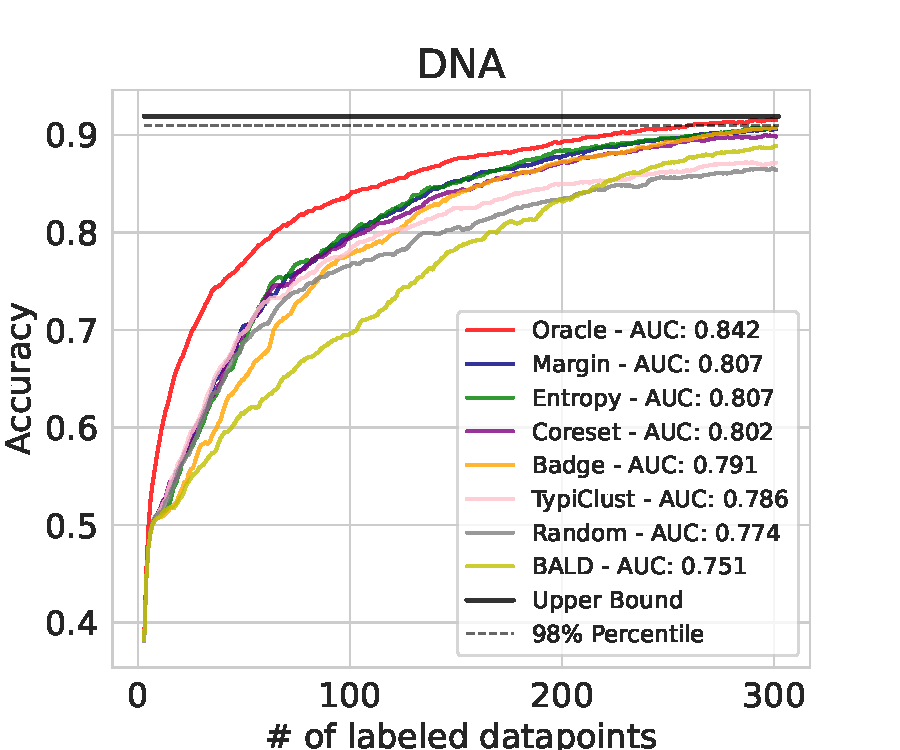
\includegraphics[width=0.49\linewidth]{img/eval_dna}
	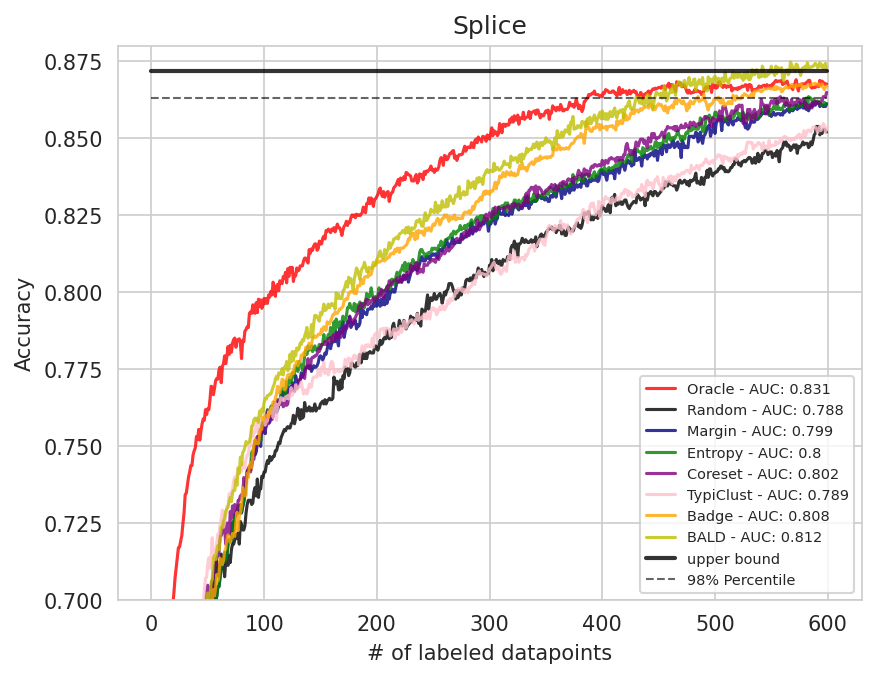
\includegraphics[width=0.49\linewidth]{img/eval_splice.png}
	\caption{Results for all algorithms on Splice and DNA, both from the tabular domain. Even within one domain, the performance of the same algorithm can vary drastically.}
	\label{fig:eval_vector}
\end{figure}
%
\begin{figure}
\centering
	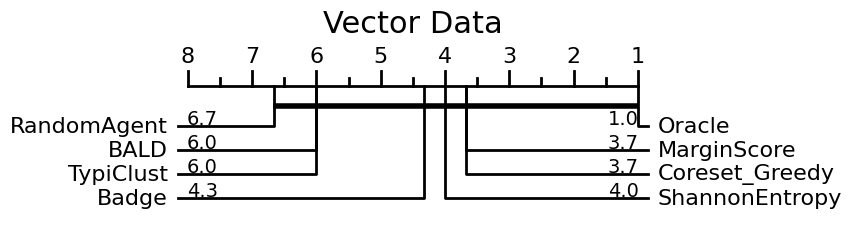
\includegraphics[width=0.49\linewidth]{img/vector.png}
	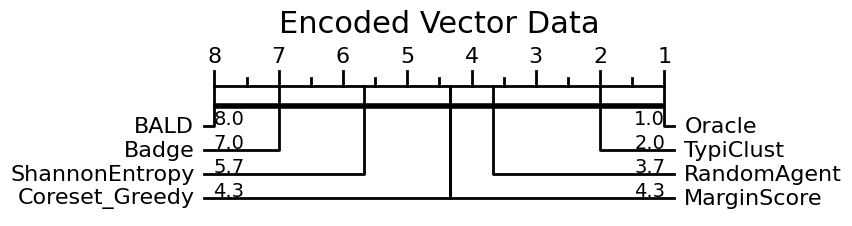
\includegraphics[width=0.49\linewidth]{img/vector_enc.png}
	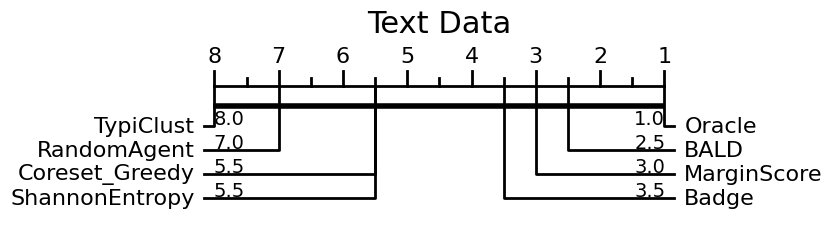
\includegraphics[width=0.49\linewidth]{img/text.png}
	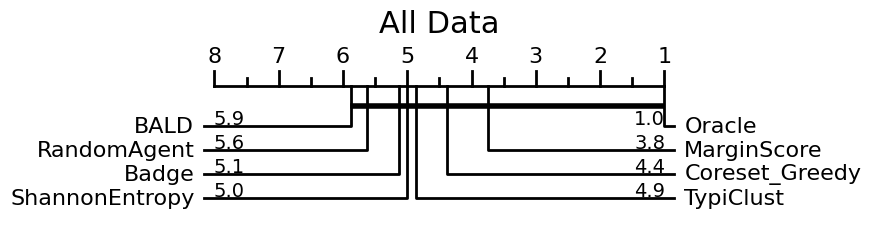
\includegraphics[width=0.49\linewidth]{img/all_data.png}
	\caption{Critical Difference Diagram for all algorithms grouped by domain and all domains combined. Ranks are computed based on median AUC for each algorithm and dataset combination. Lower ranks are better.}
	\label{fig:cd_diagrams}
\end{figure}
%
From Fig. \ref{fig:eval_vector} we notice drastically different qualities for the same AL algorithm for different datasets.
We would like to highlight that both datasets are tabular from the medical domain with similar number of features and classes, yet we see that i.e. BALD is the best algorithm for Splice and the worst algorithm for DNA.
These inconsistencies are present between the datasets of all our tested domains, further highlighting the difficulties for comparing AL algorithms in terms of average performance.
In order to provide a meaningful analysis of which algorithm can be expected to perform best on average we ranked the algorithm for each dataset based on their median AUC and displayed these rankings in critical difference diagrams \cite{IsmailFawaz2018deep}.
In Fig. \ref{fig:cd_diagrams} we report the rankings split by domain as well as across all domains (excluding the toydata).

\section{Conclusion}

\section{Limitations and Future Work}
No batch AL \\
No learned algorithms \\
No improved classifier training (semi-supervised, etc.)

\newpage

\bibliographystyle{plain}
\bibliography{main.bib} 

\appendix

\section{Other result tables}
\begin{table}[H]
	\begin{tabular}{l|lll}
		& SpliceEncoded & DNAEncoded    & USPSEncoded   \\
		\hline
		Oracle          & 0.754 +- 0.02 & 0.726 +- 0.02 & 0.674 +- 0.01 \\
		SAL & 0.675 +- 0.03 & 0.640 +- 0.04 & 0.634 +- 0.01 \\
		Coreset & 0.690 +- 0.02 & 0.644 +- 0.05 & 0.607 +- 0.02 \\
		TypiClust       & 0.695 +- 0.02 & 0.660 +- 0.03 & 0.643 +- 0.01 \\
		MarginScore     & 0.675 +- 0.03 & 0.643 +- 0.05 & 0.632 +- 0.02 \\
		ShannonEntropy  & 0.673 +- 0.03 & 0.638 +- 0.05 & 0.626 +- 0.02 \\
		RandomAgent     & 0.680 +- 0.03 & 0.633 +- 0.04 & 0.594 +- 0.02 \\
		Badge           & 0.670 +- 0.04 & 0.600 +- 0.07 & 0.597 +- 0.02 \\
		BALD            & 0.660 +- 0.04 & 0.597 +- 0.06 & 0.652 +- 0.01
	\end{tabular}
	\caption{AUC values for all algorithms on the encoded tabular datasets. Higher is better.}
\end{table}
%
\begin{table}[H]
	\begin{tabular}{l|ll}
		& Cifar10Encoded & FashionMnistEncoded \\
		\hline
		Oracle          & 0.699 +- 0.01  & 0.721 +- 0.01       \\
		SAL & 0.623 +- 0.01  & 0.667 +- 0.01       \\
		Coreset & 0.641 +- 0.01  & 0.674 +- 0.01       \\
		TypiClust       & 0.627 +- 0.01  & 0.638 +- 0.01       \\
		MarginScore     & 0.641 +- 0.01  & 0.676 +- 0.01       \\
		ShannonEntropy  & 0.637 +- 0.02  & 0.680 +- 0.01       \\
		RandomAgent     & 0.598 +- 0.02  & 0.633 +- 0.01       \\
		Badge           & 0.645 +- 0.02  & 0.681 +- 0.01       \\
		BALD            & 0.633 +- 0.01  & 0.666 +- 0.01      
	\end{tabular}
	\caption{AUC values for all algorithms on the encoded image datasets. Higher is better.}
\end{table}
%
\begin{table}[H]
	\begin{tabular}{l|ll}
		& TopV2         & News          \\
		\hline
		Oracle          & 0.860 +- 0.01 & 0.448 +- 0.01 \\
		SAL & 0.831 +- 0.01 & 0.312 +- 0.01 \\
		Coreset & 0.816 +- 0.02 & 0.355 +- 0.02 \\
		TypiClust       & 0.718 +- 0.02 & 0.314 +- 0.01 \\
		MarginScore     & 0.821 +- 0.02 & 0.357 +- 0.01 \\
		ShannonEntropy  & 0.794 +- 0.02 & 0.342 +- 0.01 \\
		RandomAgent     & 0.776 +- 0.02 & 0.349 +- 0.01 \\
		Badge           & 0.824 +- 0.01 & 0.343 +- 0.01 \\
		BALD            & 0.825 +- 0.02 & 0.347 +- 0.01
	\end{tabular}
\caption{AUC values for all algorithms on the text datasets. Higher is better.}
\end{table}

\section{Alternative Plot for Restarts Ablation}
\begin{figure}[H]
	\centering
	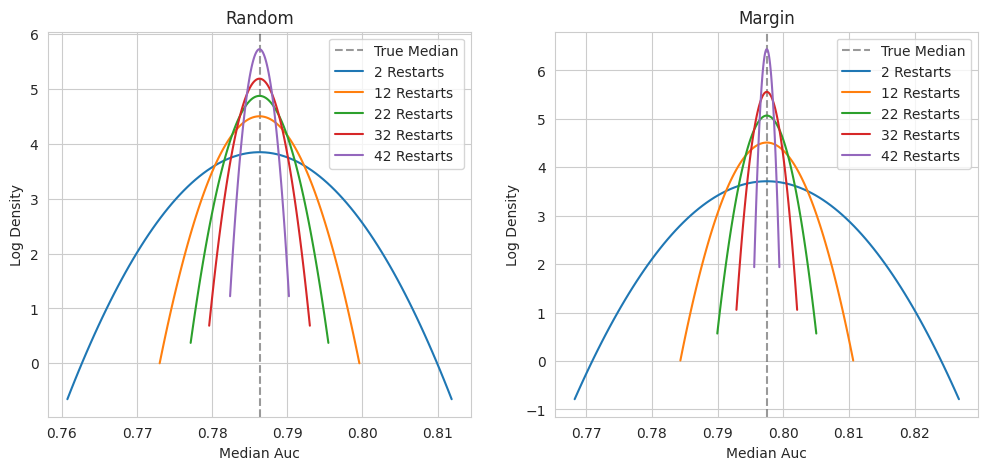
\includegraphics[width=\linewidth]{img/ablation_restarts_2.png}
\end{figure}

\section{Hyperparameters per Dataset}\label{app:hyperparameters}
\begin{table}[H]
	\centering
	\begin{tabular}{l || l | l l l l}
		Dataset & Classifier & Optimizer & LR & Weight Decay & Dropout \\
		\hline
		Splice & [24, 12] & NAdam & 1.2e-3 & 5.9e-5 & 0 \\
		SpliceEnc. & linear & NAdam & 6.2e-4 & 5.9e-6 & 0 \\
		DNA & [24, 12] & NAdam & 3.9e-2 & 3.6e-5 & 0 \\
		DNAEnc & linear & NAdam & 1.6e-3 & 4e-4 & 0 \\
		USPS & [24, 12] & Adam & 8.1e-3 & 1.5e-6 & 0 \\
		USPS & linear & NAdam & 7.8e-3 & 1.9e-6 & 0 \\
		FashionMnist & ResNet18 & NAdam & 1e-3 & 0 & 0 \\
		FashionMnistEnc & linear & Adam & 1.6e-3 & 1e-5 & 5e-2 \\
		Cifar10 & ResNet18 & NAdam & 1e-3 & 0 & 0 \\
		Cifar10Enc & linear & NAdam & 1.7e-3 & 2.3e-5 & 0 \\
		TopV2 & BiLSTM & NAdam & 1.5e-3 & 1.7e-7 & 5e-2 \\
		News & BiLSTM & NAdam & 1.5e-3 & 1.7e-7 & 5e-2 \\
	\end{tabular}
	\caption{Classifier architectures and optimized hyperparameters per dataset. Numbers in brackets signify a MLP with corresponding hidden layers.}
	\label{tab:architectures}
\end{table}


\section{Comparison of different sample sizes}
\begin{figure}[H]
\centering
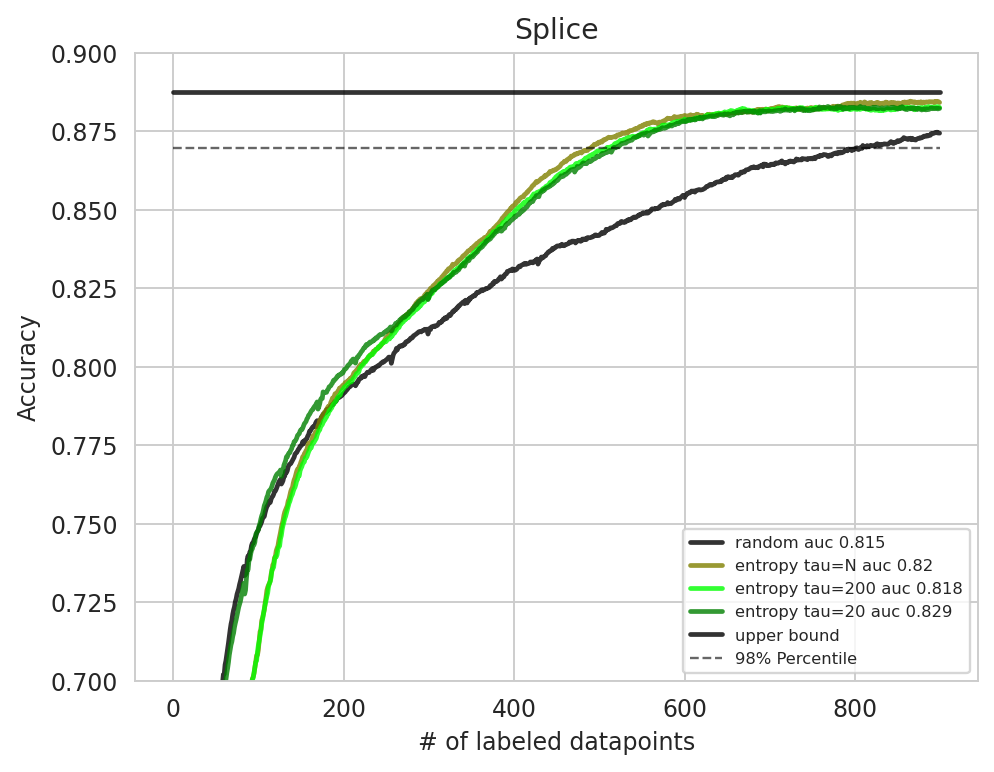
\includegraphics[width=0.7\linewidth]{img/tau_ablation.png}
\end{figure}

\section{AL Pseudocode}
\begin{algorithm}[H]
	\caption{Active Learning}\label{alg:active_learning}
	\begin{algorithmic}[1]
		\Require $\mathcal{U}$ \Comment{Unlabeled Pool}
		\Require $\tau$ \Comment{Unlabeled Sample Size}
		\Require $\Omega$ \Comment{AL Agent}
		\Require $\omega$ \Comment{Environment State function}
		\State $\mathcal{L}^{(1)} \gets \operatorname{seed}(\mathcal{U})$  \Comment{Create the initial labeled set}
		\State $\mathcal{U}^{(1)} \gets \mathcal{U}$
		\For{$i := 1 \ldots B$}
		\State $\text{acc}^{(i)} \gets \operatorname{Retrain}(\mathcal{L}^{(i)})$  %\Comment{$\operatorname{Retrain}(\mathcal{L}^{(i)})$ is shorthand for $\operatorname{Retrain}(\mathcal{L}^{(i)}, \mathcal{L}^\text{test}, \hat y_\theta, e^\text{max})$}
		%\State $u^{(i)} \sim \text{unif}(1:|\mathcal{U}^{(i)}|)$
		\State $a^{(i)} \gets \Omega(\mathcal{U}^{(i)}) \hspace{1mm};\hspace{2mm} a \in 1:|\mathcal{U}^{(i)}|$ 
		%\Comment{$a^{(i)}$ is an index inside of $u^{(i)}$}
		\State $y^{(i)} \gets \operatorname{label}(\mathcal{U}^{(i)}_{a})$ 
		%\Comment{$u^{(i)}_{a}$ is shorthand for $u^{(i)}_{a^{(i)}}$}
		\State $\mathcal{L}^{(i+1)} \gets \mathcal{L}^{(i)} \cup \{(\mathcal{U}^{(i)}_a, y^{(i)})\}$
		\State $\mathcal{U}^{(i+1)} \gets \mathcal{U}^{(i)} \setminus \{\mathcal{U}^{(i)}_a\}$
		\EndFor
		\State
		\Return $\frac{1}{B} \sum_{i=1}^{B} \text{acc}^{(i)}$
	\end{algorithmic}
\end{algorithm}

\end{document}
